% Paquets généraux
\documentclass[a4paper,12pt,titlepage]{article}
\usepackage[T1]{fontenc}
\usepackage[utf8]{inputenc}
\usepackage[french]{babel}
\usepackage[gen]{eurosym}
%\usepackage[dvips]{graphicx}
\usepackage{fancyhdr}
\usepackage{pdfpages} 
\usepackage{multido}
\usepackage{hyperref}
%\usepackage{textcomp}
%\usepackage{aeguill}
\usepackage{schemabloc}
\usepackage[bitstream-charter]{mathdesign}
\usepackage{minted}

\newcommand{\id}{71}
\newcommand{\nom}{Théorie des mécanismes}
\newcommand{\sequence}{04}
\newcommand{\nomsequence}{Liaisons entre les solides}
\newcommand{\num}{02}
\newcommand{\type}{KH}
\newcommand{\descrip}{Liaisons équivalentes, hyperstatisme, liaisons en série et en parallèle, théorie des graphes}
\newcommand{\competences}{B2-12: Proposer une modélisation des liaisons avec leurs caractéristiques géométriques. \\ &  B2-13: Proposer un modèle cinématique paramétré à partir d'un système réel, d'une maquette numérique ou d'u \\ &  B2-17: Simplifier un modèle de mécanisme. \\ &  B2-18: Modifier un modèle pour le rendre isostatique. \\ &  C1-04: Proposer une démarche permettant d'obtenir une loi entrée-sortie géométrique.  \\ &  C2-05: Caractériser le mouvement d'un repère par rapport à un autre repère. \\ &  C2-06: Déterminer les relations entre les grandeurs géométriques ou cinématiques. }
\newcommand{\nbcomp}{7}
\newcommand{\systemes}{}
\newcommand{\systemesnum}{}
\newcommand{\systemessansaccent}{}
\newcommand{\ilot}{2}
\newcommand{\ilotstr}{02}
\newcommand{\dossierilot}{\detokenize{Ilot_02 }}


\newcommand{\auteurun}{Renaud Costadoat}
\newcommand{\auteurdeux}{Françoise Puig}
\newcommand{\institute}{Lycée Dorian}


\usepackage{color}
\usepackage{xcolor}
\usepackage{colortbl}
\usepackage{helvet}
\usepackage[frenchmath]{newtxsf} % for sans serif symbols
\renewcommand{\familydefault}{\sfdefault}
%\usepackage{amsfonts}
%\usepackage{amsmath}
%\usepackage{lmodern}
\usepackage{mathastext}
%\usepackage{xspace}
\usepackage{varioref}
\usepackage{tabularx}
%\usepackage{floatflt}
\usepackage{graphics}
\usepackage{wrapfig}
\usepackage{textcomp}
\usepackage{tikz}
\usepackage{wrapfig}
\usepackage{gensymb}
\usepackage[european]{circuitikz}
\usetikzlibrary{babel}
\usepackage{ifthen}
\usepackage{cancel}
\usepackage{etoolbox}
\usepackage{multirow}
%\usepackage{boxedminipage}
\definecolor{gris25}{gray}{0.75}
\definecolor{bleu}{RGB}{18,33,98}
\definecolor{bleuf}{RGB}{42,94,171}
\definecolor{bleuc}{RGB}{231,239,247}
\definecolor{rougef}{RGB}{185,18,27}
\definecolor{rougec}{RGB}{255,188,204}%255,230,231
\definecolor{vertf}{RGB}{103,126,82}
\definecolor{vertc}{RGB}{220,255,191}
\definecolor{forestgreen}{rgb}{0.13,0.54,0.13}
\definecolor{blcr}{rgb}{0.59,0.69,0.84}
\definecolor{blfr}{rgb}{0.32,0.51,0.75}
\definecolor{orfr}{rgb}{0.90,0.42,0.15}
\definecolor{orcr}{rgb}{0.90,0.65,0.50}
\definecolor{orangef}{rgb}{0.659,0.269,0.072}
\definecolor{orange}{rgb}{0.58,0.35,0.063}
\definecolor{orangec}{rgb}{0.43,0.32,0.25}
\definecolor{rcorrect}{rgb}{0.6,0,0}
\definecolor{sequence}{rgb}{0.75,0.75,0.75}
\definecolor{competences}{rgb}{0.61,0.73,0.35}
\definecolor{grisf}{HTML}{222222}
\definecolor{grisc}{HTML}{636363}
\definecolor{normal}{HTML}{4087c4}
\definecolor{info}{HTML}{5bc0de}
\definecolor{success}{RGB}{92,184,92}
\definecolor{warning}{RGB}{240,173,78}
\definecolor{danger}{RGB}{217,83,79}
\hypersetup{                    % parametrage des hyperliens
    colorlinks=true,                % colorise les liens
    breaklinks=true,                % permet les retours à la ligne pour les liens trop longs
    urlcolor= blfr,                 % couleur des hyperliens
    linkcolor= orange,                % couleur des liens internes aux documents (index, figures, tableaux, equations,...)
    citecolor= forestgreen                % couleur des liens vers les references bibliographiques
    }

% Mise en page
\pagestyle{fancy}

\setlength{\hoffset}{-18pt}

\setlength{\oddsidemargin}{0pt} 	% Marge gauche sur pages impaires
\setlength{\evensidemargin}{0pt} 	% Marge gauche sur pages paires
\setlength{\marginparwidth}{00pt} 	% Largeur de note dans la marge
\setlength{\headwidth}{481pt} 	 	% Largeur de la zone de tête (17cm)
\setlength{\textwidth}{481pt} 	 	% Largeur de la zone de texte (17cm)
\setlength{\voffset}{-18pt} 		% Bon pour DOS
\setlength{\marginparsep}{7pt}	 	% Séparation de la marge
\setlength{\topmargin}{-30pt} 		% Pas de marge en haut
\setlength{\headheight}{35pt} 		% Haut de page
\setlength{\headsep}{20pt} 		% Entre le haut de page et le texte
\setlength{\footskip}{30pt} 		% Bas de page + séparation
\setlength{\textheight}{700pt} 		% Hauteur de l'icone zone de texte (25cm)
\setlength\fboxrule{1 pt}
\renewcommand{\baselinestretch}{1}
\setcounter{tocdepth}{1}
\newcommand{\cadre}[2]
{\fbox{
  \begin{minipage}{#1\linewidth}
   \begin{center}
    #2\\
   \end{center}
  \end{minipage}
 }
}

\newcounter{num_quest} \setcounter{num_quest}{0}
\newcounter{num_rep} \setcounter{num_rep}{0}
\newcounter{num_cor} \setcounter{num_cor}{0}

\newcommand{\question}[1]{\refstepcounter{num_quest}\par
~\ \\ \parbox[t][][t]{0.15\linewidth}{\textbf{Question \arabic{num_quest}}}\parbox[t][][t]{0.93\linewidth}{#1}\par
}


\newcommand{\reponse}[1]
{\refstepcounter{num_rep}
\noindent
\rule{\linewidth}{.5pt}
\textbf{Question \arabic{num_rep}:}
\multido{\i=1+1}{#1}{~\ \\}
}

\newcommand{\cor}
{\refstepcounter{num_cor}
\noindent
\rule{\linewidth}{.5pt}
\textbf{Question \arabic{num_cor}:} \\
}

\newcommand{\titre}[1]
{\begin{center}
\cadre{0.8}{\huge #1} 
\end{center}
}


% En tête et pied de page
\fancypagestyle{normal}{%
  \fancyhf{}
\lhead{\nom}
\rhead{
\includegraphics[width=2cm]{../../img/logo}\hspace{2pt}}
\ifdef{\auteurdeux}{\lfoot{\auteurun,\auteurdeux}}{\lfoot{\auteurun}}
\cfoot{Page \thepage}}

\fancypagestyle{correction}{%
  \fancyhf{}
  \lhead{\colorbox{danger}{\begin{minipage}{0.65\paperwidth} \textcolor{white}{\textbf{Correction}} \end{minipage}} }
  \rhead{
\includegraphics[width=2cm]{../../img/logo}}
  \ifdef{\auteurdeux}{\lfoot{\auteurun,\auteurdeux}}{\lfoot{\auteurun}}
  \rfoot{\colorbox{danger}{\begin{minipage}{0.5\paperwidth} \begin{flushright}\textcolor{white}{\textbf{Correction}}\end{flushright} \end{minipage}} }}

\renewcommand{\footrulewidth}{0.4pt}

\usepackage{eso-pic}
\newcommand{\BackgroundPic}{%
\put(0,0){%
\parbox[b][\paperheight]{\paperwidth}{%
\vfill
\begin{center}
\hspace{0.5cm}\vspace{0.5cm}
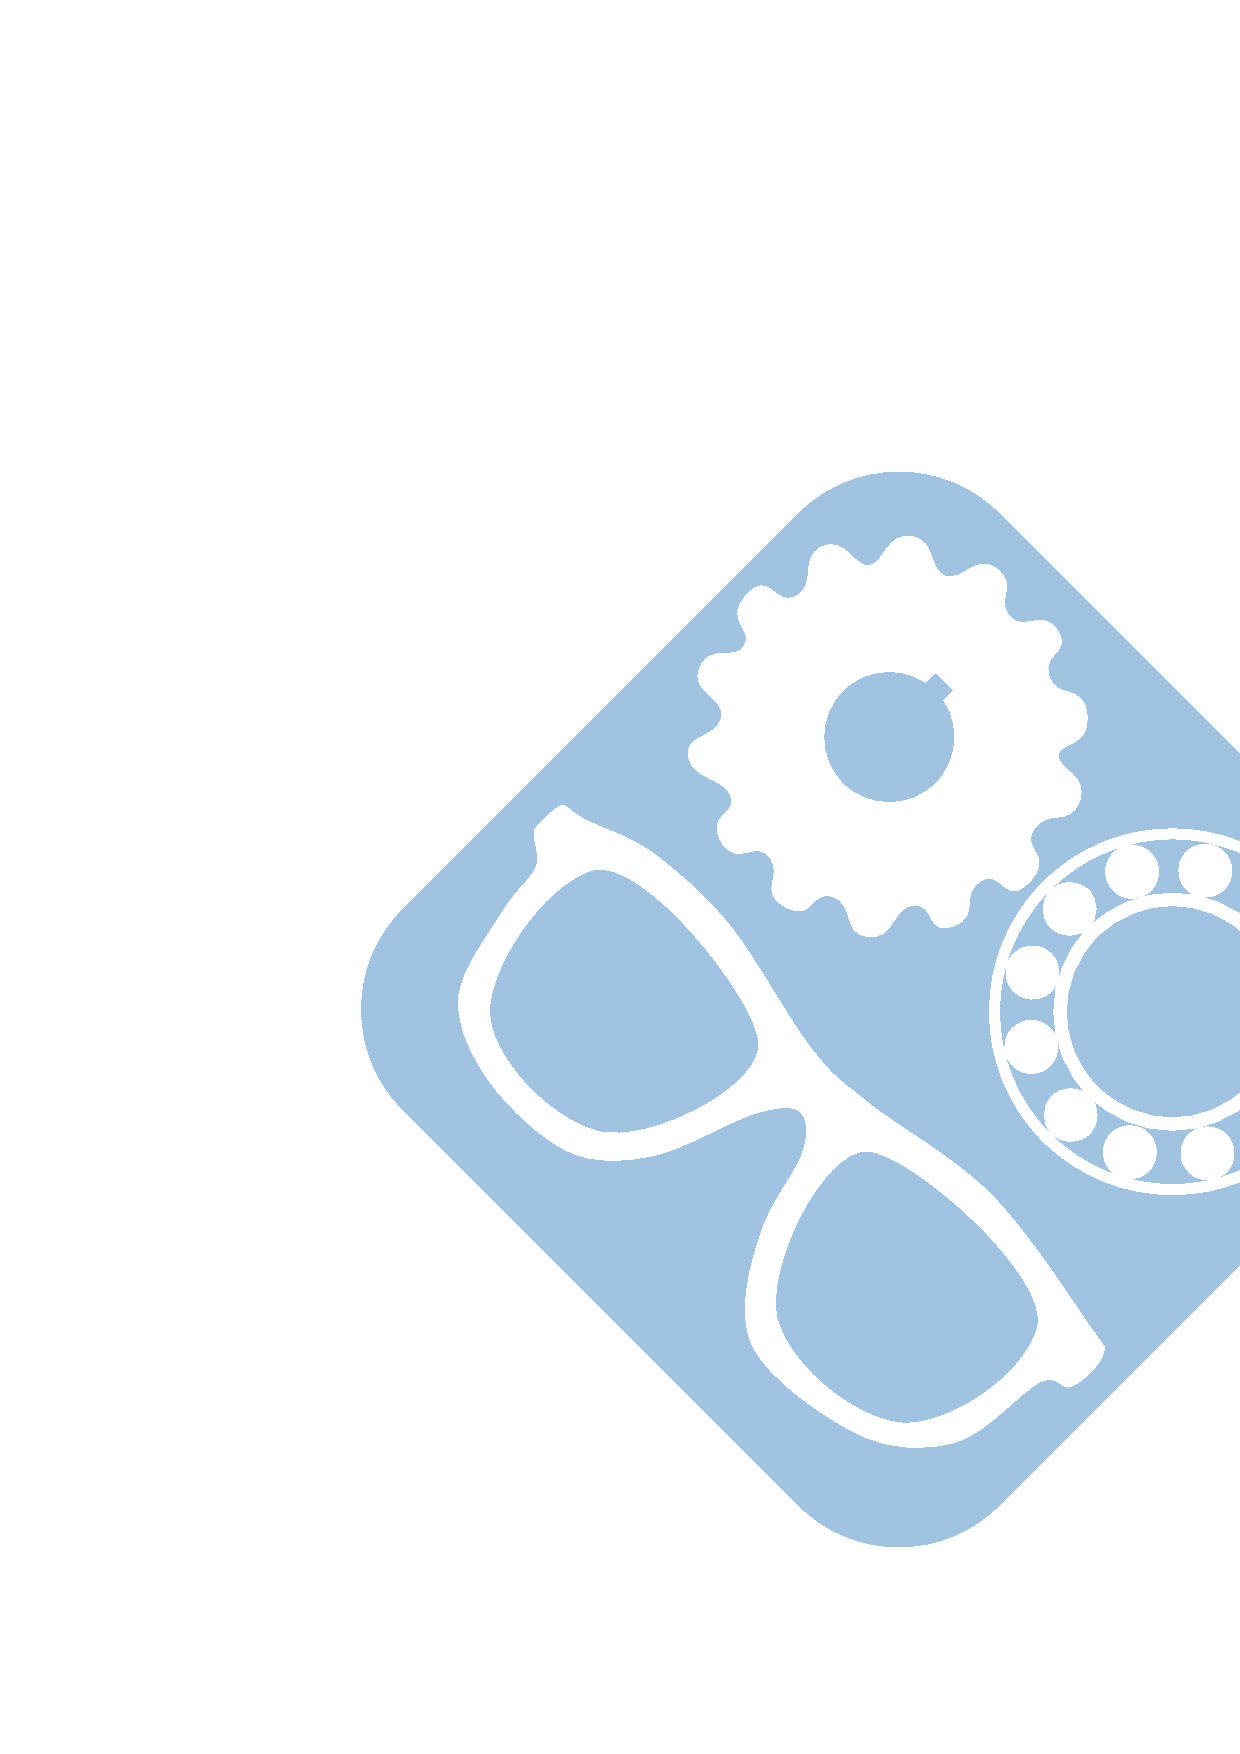
\includegraphics[width=\paperwidth,height=\paperheight,%
keepaspectratio]{../../img/fond3}%
\end{center}
\vfill
}}}

\newcommand{\BackgroundPicdeux}{%
\put(25,-30){%
\parbox[b][\paperheight]{\paperwidth}{%
\vfill
\begin{center}
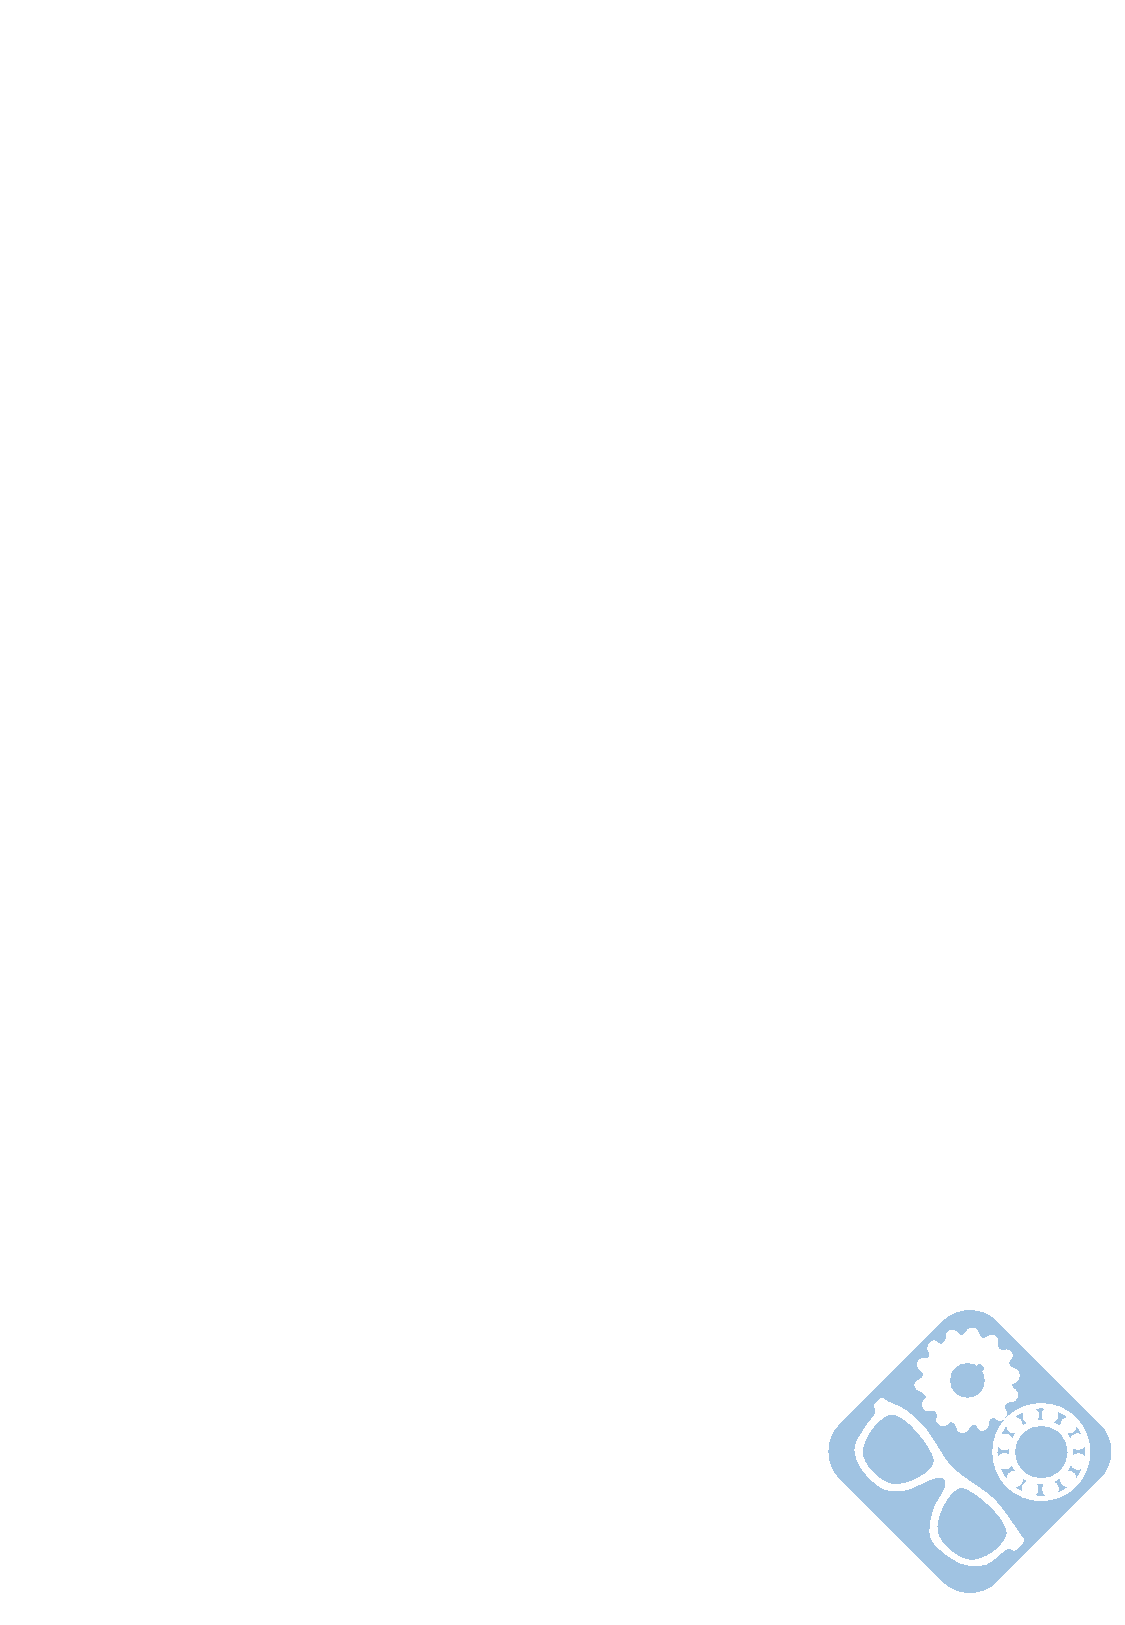
\includegraphics[width=\paperwidth,height=\paperheight,%
keepaspectratio]{../../img/fond4}%
\end{center}
\vfill
}}}

\begin{document}

\pagestyle{empty}

\vspace*{-3\baselineskip}

\AddToShipoutPicture*{\BackgroundPic}

\ifdef{\auteurdeux}{\begin{tabular}{>{\columncolor{gray!00}}m{.3\linewidth} m{.3\linewidth} >{\columncolor{gray!00}}m{.3\linewidth}}
Séquence : \sequence &  \multirow{3}{*}{\hspace{1cm}
\includegraphics[height=1.5cm]{../../img/logo}} &  \begin{flushright} \multirow{4}{*}{\hspace{1cm}\includegraphics[height=4cm]{img/qrcode}}\end{flushright}\\
Document : \type\num \\
 \institute \\
 \auteurun\\
 \auteurdeux
\end{tabular}}{\begin{tabular}{>{\columncolor{gray!00}}m{.3\linewidth} m{.3\linewidth} >{\columncolor{gray!00}}m{.3\linewidth}}
Séquence : \sequence &  \multirow{3}{*}{\hspace{1cm}
\includegraphics[height=1.5cm]{../../img/logo}} &  \begin{flushright} \multirow{4}{*}{\hspace{1cm}\includegraphics[height=4cm]{img/qrcode}}\end{flushright}\\
Document : \type\num \\
 \institute \\
 \auteurun
\end{tabular}}

\vspace{1cm}

\ifdef{\prive}{\begin{center}\colorbox{danger}{\Huge{Avec Correction}}\end{center}}{}

\begin{center}\huge{\nom}\end{center}

\vspace{2cm}

\ifdef{\imagedeux}{\begin{minipage}{0.49\linewidth}}{}
\begin{center}\includegraphics[height=5cm]{/home/renaud/Documents/Renaud/GitHub/django_education/systemes/\imageun}\end{center}
\ifdef{\imagedeux}{\end{minipage}\hfill
\begin{minipage}{0.49\linewidth}
\begin{center}\includegraphics[height=5cm]{/home/renaud/Documents/Renaud/GitHub/django_education/systemes/\imagedeux}\end{center}
\end{minipage}}{}

\vspace{5cm}


\begin{tabular}{p{.15\linewidth} >{\columncolor{white}}p{.8\linewidth}}
    \rowcolor{gray!20}
    Référence & S\sequence\ - \type\num \\
    Compétences & \competences \\
 	\rowcolor{gray!20}
    Description & \descrip \\
    Système & \systemes
  \end{tabular}

\newpage

\AddToShipoutPicture{\BackgroundPicdeux}

\pagestyle{normal}

\section{Machine d'essai universelle EM 550}

La machine électromécanique universelle EM 550, figure \ref{fig:image3} est conçue pour être utilisée dans de nombreuses applications d'essais de matériaux et de structures. Elle permet de réaliser des essais de traction, de compression, de flexion, de fatigue, de fluage, de dureté, de frottement ainsi que des tests sur des assemblages et des structures. Cette machine est commercialisée par DELTALAB. Elle est présente dans les laboratoires des services recherche et développement de nombreuses entreprises.

La machine d'essais est reliée à un micro-ordinateur équipé du logiciel DELTALAB, d'une interface logiciel/machine pour le pilotage, l'acquisition et le traitement des données et d'une imprimante.

\begin{figure}[htbp]
\begin{minipage}[c]{.40\linewidth}
\begin{center}
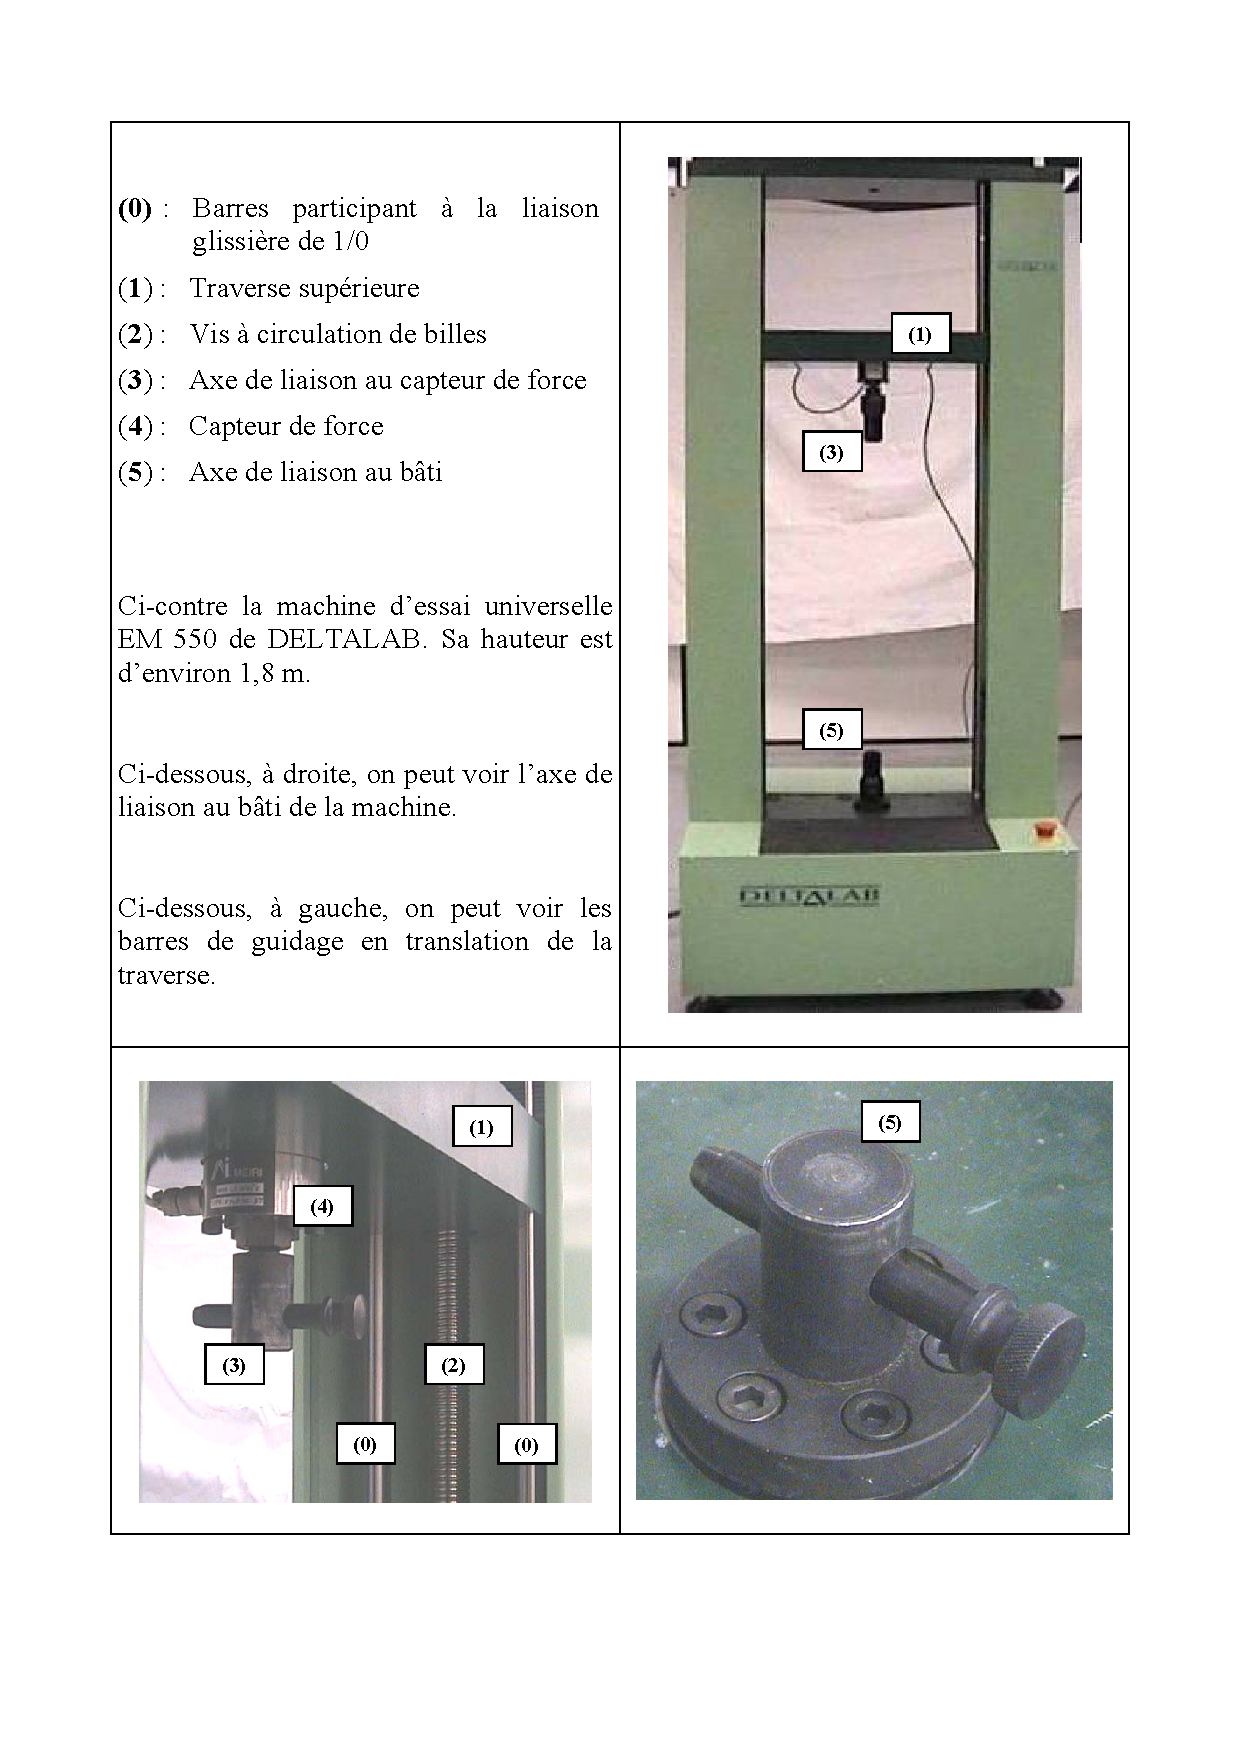
\includegraphics[width=\linewidth]{img/annexe1.pdf}
\caption{Machine EM 550}
\label{fig:image3}
\end{center}
\end{minipage}
\hfill
\begin{minipage}[c]{.55\linewidth}
Caractéristiques générales (voir schéma cinématique en annexe 2) :
\begin{itemize}
 \item Effort maximal sur la traverse : 50 kN.
 \item Course maximale : 1 m.
 \item Entraînement : servomoteur à courant continu avec génératrice tachymétrique.
 \item Transmission : réducteur roue et vis sans fin, poulies, courroie crantée et vis et écrous à billes.
 \item Mesure du déplacement : codeur optoélectronique de résolution 500 positions par tour.
 \item Mesure de l'effort : capteur à jauges de déformations.
 \item Alimentation : 240 V monophasé / 50 Hz - 1 kW max.
 \item Couple permanent du servomoteur : 3 N.m,
 \item $\overrightarrow{AA'}=2.e.\overrightarrow{x}$.
\end{itemize}
\end{minipage}
\end{figure}

La traverse est liée au bâti par deux liaisons glissières montées en parallèle.

Le schéma cinématique du montage est donné sur la figure \ref{fig:image4}.

\begin{figure}[htbp]
\begin{center}
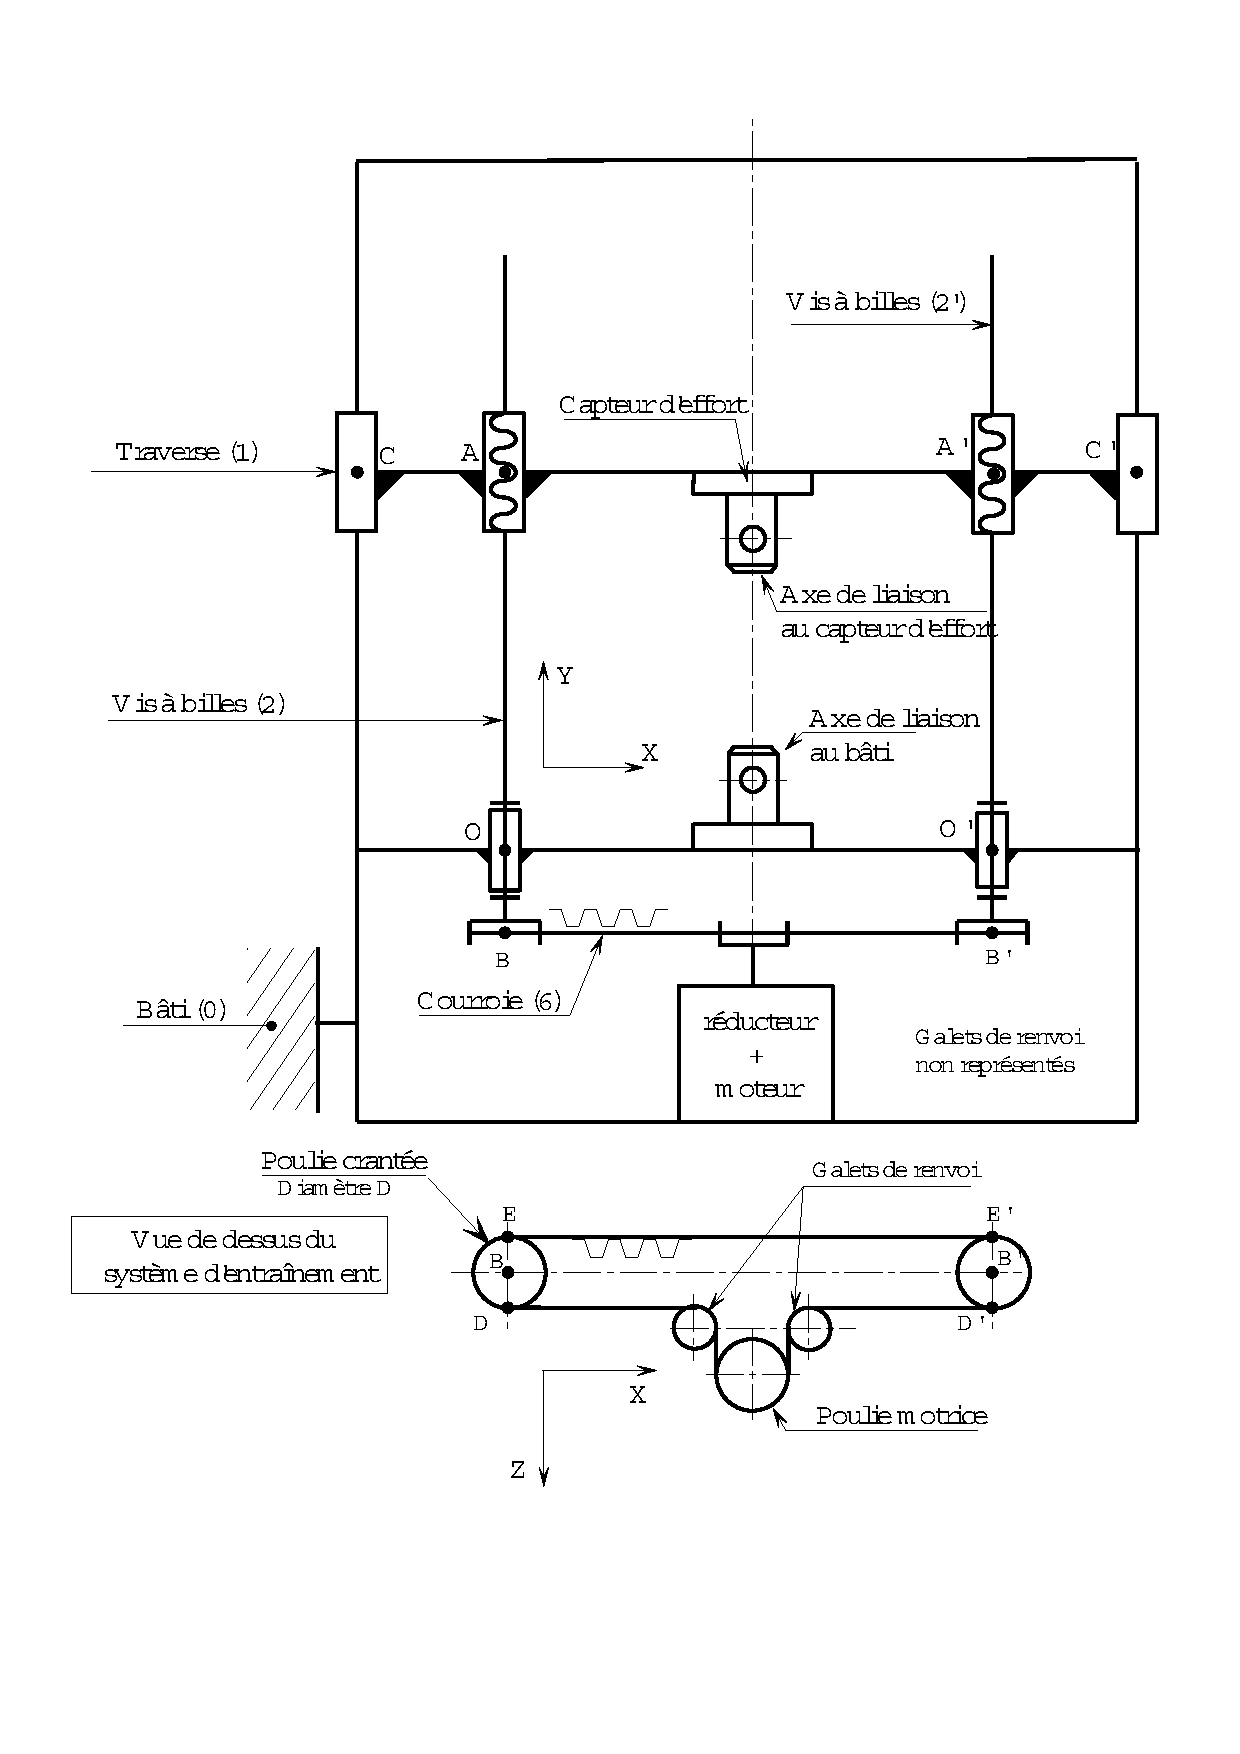
\includegraphics[width=0.7\linewidth]{img/cin_EM.pdf}
\caption{Schéma cinématique}
\label{fig:image4}
\end{center}
\end{figure}

\paragraph{Question 1:}

Modéliser le mécanisme grâce à un graphe de liaisons.

\paragraph{Question 2:}

Déterminer le degré d'hyperstatisme de ce mécanisme.

\paragraph{Question 3:}

Valider ce résultat en effectuant une étude sur les équations issues des torseurs cinématiques. A partir du système d'équations proposé, proposer des modifications qui permettraient de le rendre isostatique.

\newpage

\section{Système E.P.A.S.}

\subsection{Introduction}

\begin{figure}[htbp]
\begin{minipage}[c]{.55\linewidth}
Une E.P.A.S. est une Echelle Pivotante Automatique à commande Séquentielle. Ce système est monté sur le châssis d'un camion de pompiers et permet de déplacer une plate forme pouvant recevoir deux personnes et un brancard le plus rapidement possible et en toute sécurité.
\end{minipage}
\hfill
\begin{minipage}[c]{.40\linewidth}
\begin{center}
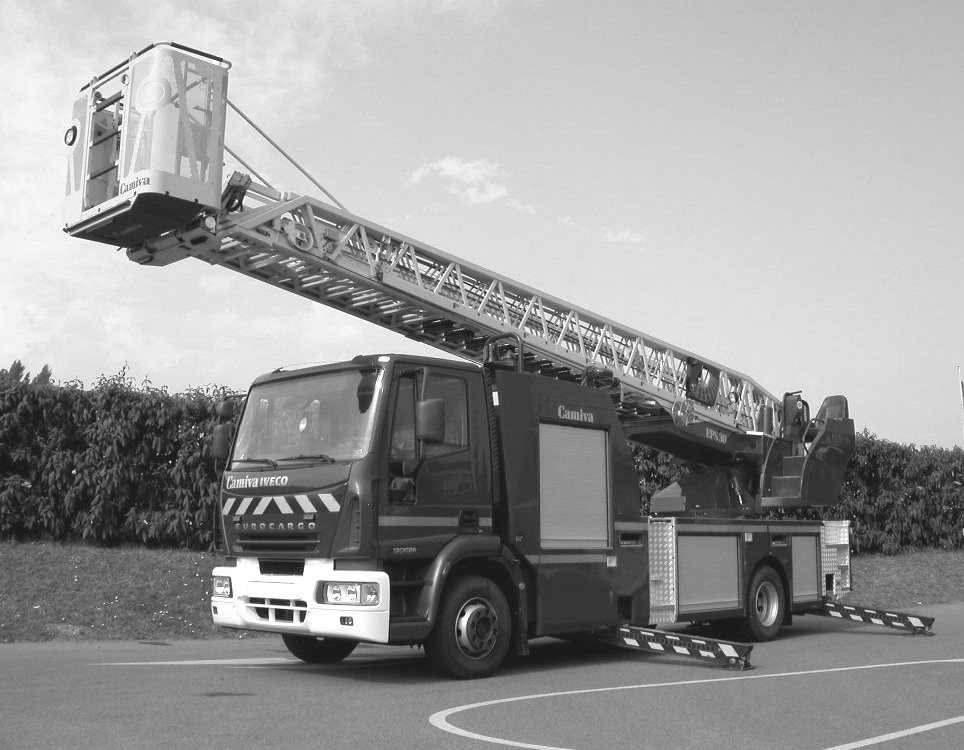
\includegraphics[width=0.8\linewidth]{img/photo_camion.jpg}
\caption{Système E.P.A.S.}
\label{fig:image1}
\end{center}
\end{minipage}
\end{figure}

La figure \ref{fig:image2} donne un schéma cinématique du système de man\oe uvre du parc échelle.

\begin{figure}[htbp]
\begin{center}
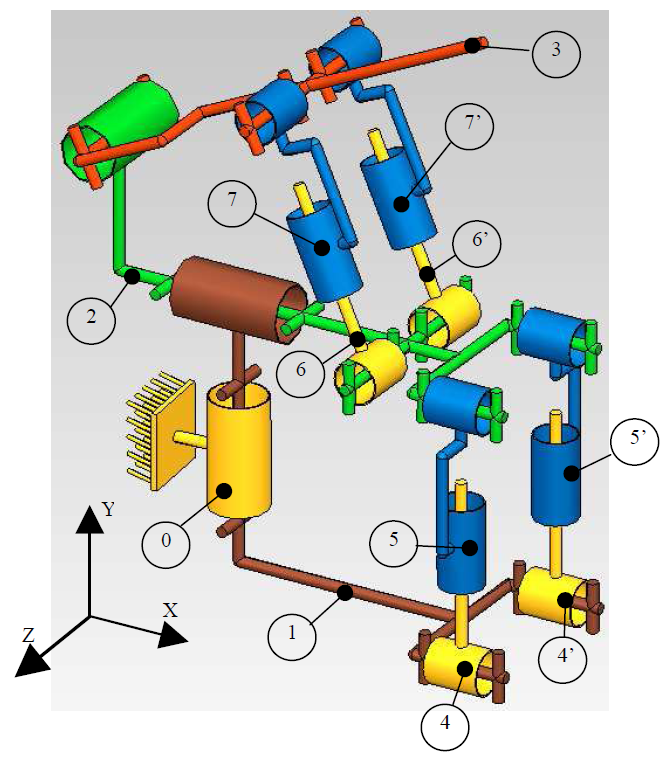
\includegraphics[width=0.4\linewidth]{img/epas_hyp.png}
\caption{Schéma cinématique du système de man\oe uvre}
\label{fig:image2}
\end{center}
\end{figure}

\paragraph{Question 1:}

Modéliser le mécanisme grâce à un graphe de liaisons.

\paragraph{Question 2:}

Déterminer le degré d'hyperstatisme de ce mécanisme.

\paragraph{Question 3:}

Valider ce résultat en effectuant une étude sur les équations issues des torseurs cinématiques. A partir du système d'équations proposé, proposer des modifications qui permettraient de le rendre isostatique.

\clearpage

\ifdef{\public}{\end{document}}{}

\newpage

\pagestyle{correction}\setcounter{section}{0}

\section{Correction}

\subsection{Machine d'essai universelle EM 550}

\paragraph{Question 1:} Liaisons du mécanisme:
\begin{enumerate}
 \item Liaison glissière en C entre 1 et 0 (direction $\overrightarrow{y}$),
 \item Liaison glissière en C' entre 1 et 0 (direction $\overrightarrow{y}$),
 \item Liaison pivot entre 2 et 0 (axe O,$\overrightarrow{y}$),
 \item Liaison pivot entre 2' et 0 (axe O',$\overrightarrow{y}$),
 \item Liaison hélicoïdale entre 2 et 1 (axe A,$\overrightarrow{y}$),
 \item Liaison hélicoïdale entre 2' et 1 (axe A',$\overrightarrow{y}$).
\end{enumerate}

\paragraph{Question 2:} Calcul d'hyperstatisme:
\begin{itemize}
 \item $4$ pièces dont le bâti,
 \item $30$ inconnues de liaison,
 \item les pièces flexibles (courroie) ne sont pas prises en compte,
 \item le système possède une mobilité.
\end{itemize}

h=Ns-rs=30-(6*3-1)=13

~\

\textbf{Le degré d'hyperstatisme du système est 13}.

\paragraph{Question 3:} 
$\left\{V_{1/0}\right\}=\left\{\begin{array}{c c} 0 & 0 \\ 0 & V_{10} \\ 0 & 0
\end{array}\right\}_{(C,R)}$,
$\left\{V'_{1/0}\right\}=\left\{\begin{array}{c c} 0 & 0 \\ 0 & V'_{10} \\ 0 & 0
\end{array}\right\}_{(C',R)}$,
$\left\{V_{2/0}\right\}=\left\{\begin{array}{c c} 0 & 0 \\ \omega_{20} & 0 \\ 0 & 0
\end{array}\right\}_{(O,R)}$,
$\left\{V'_{2/0}\right\}=\left\{\begin{array}{c c} 0 & 0 \\ \omega'_{2'0} & 0 \\ 0 & 0
\end{array}\right\}_{(O',R)}$,
$\left\{V_{2/1}\right\}=\left\{\begin{array}{c c} 0 & 0 \\ \omega_{21} & \dfrac{p}{2.\pi}.\omega_{21} \\ 0 & 0
\end{array}\right\}_{(A,R)}$,
$\left\{V'_{2/1}\right\}=\left\{\begin{array}{c c} 0 & 0 \\ \omega'_{2'1} & \dfrac{p}{2.\pi}.\omega'_{2'1} \\ 0 & 0
\end{array}\right\}_{(A',R)}$

~\

On peut tout ramener en A.

$\left\{V_{1/0}\right\}=\left\{\begin{array}{c c} 0 & 0 \\ 0 & V_{10} \\ 0 & 0
\end{array}\right\}_{(A,R)}$,
$\left\{V'_{1/0}\right\}=\left\{\begin{array}{c c} 0 & 0 \\ 0 & V'_{10} \\ 0 & 0
\end{array}\right\}_{(A,R)}$,
$\left\{V_{2/0}\right\}=\left\{\begin{array}{c c} 0 & 0 \\ \omega_{20} & 0 \\ 0 & 0
\end{array}\right\}_{(A,R)}$ \\
$\left\{V_{2/1}\right\}=\left\{\begin{array}{c c} 0 & 0 \\ \omega_{21} & \dfrac{p}{2.\pi}.\omega_{21} \\ 0 & 0\end{array}\right\}_{(A,R)}$,
$\left\{V'_{2/0}\right\}\left\{\begin{array}{c c} 0 & 0 \\ \omega'_{2'0} & 0 \\ 0 & 2.e.\omega'_{2'0}\end{array}\right\}_{(A,R)}$,
$\left\{V'_{2/1}\right\}=\left\{\begin{array}{c c} 0 & 0 \\ \omega'_{2'1} & \dfrac{p}{2.\pi}.\omega'_{2'1} \\ 0 & 2.e.\omega'_{2'1} \end{array}\right\}_{(A',R)}$

$\left\{\begin{array}{c c} 0 & 0 \\ 0 & V_{10} \\ 0 & 0
\end{array}\right\}_{(A,R)}=\left\{\begin{array}{c c} 0 & 0 \\ 0 & V'_{10} \\ 0 & 0
\end{array}\right\}_{(A,R)}=\left\{\begin{array}{c c} 0 & 0 \\ \omega_{20}-\omega_{21} & -\dfrac{p}{2.\pi}.\omega_{21} \\ 0 & 0
\end{array}\right\}_{(A,R)}$\\$=\left\{\begin{array}{c c} 0 & 0 \\ \omega'_{2'0}-\omega'_{2'1} & -\dfrac{p}{2.\pi}.\omega'_{2'1} \\ 0 &  2.e.(\omega'_{2'0}-\omega'_{2'1})\end{array}\right\}_{(A',R)}$

$\left\{\begin{array}{l}
0=0=0=0 \\ 
0=0=\omega_{20}-\omega_{21}=\omega'_{2'0}-\omega'_{2'1} \\
0=0=0=0 \\
0=0=0=0 \\
V_{10}=V'_{10}=-\dfrac{p}{2.\pi}.\omega_{2'1}=-\dfrac{p}{2.\pi}.\omega'_{2'1} \\
0=0=0=2.e.(\omega'_{2'0}-\omega'_{2'1})\\
\end{array}\right.$

~\

Analyse des équations:
\begin{itemize}
 \item il y a 12 équations du type $0=0$,
 \item une équation $0=2.e.(\omega'_{2'0}-\omega'_{2'1})$, identique à $0=\omega'_{2'0}-\omega'_{2'1}$,
 \item Soit un total de 13 équations non indépendantes.
\end{itemize}

Cela confirme le degré d'hyperstatisme déterminé précédemment.

~\

La suppression des deux liaisons glissières (les liaisons deviennent des liaisons à 6 degrés de liberté) donne:

$\left\{\begin{array}{l}
\omega_{10x}=\omega'_{10x}=0=0 \\ 
\omega_{10y}=\omega'_{10y}=\omega_{20}-\omega_{21}=\omega'_{20}-\omega'_{21} \\
\omega_{10z}=\omega'_{10z}=0=0 \\
V_{10x}=V'_{10x}=0=0 \\
V_{10}=V'_{10}=-\dfrac{p}{2.\pi}.\omega_{21}=-\dfrac{p}{2.\pi}.\omega'_{21} \\
V_{10z}=V'_{10z}=0=2.e.(\omega'_{20}-\omega'_{21})\\
\end{array}\right.$

~\

Le remplacement de la liaison pivot en A' par une linéaire annulaire d'axe (A',$\overrightarrow{x}$) donne:

$\left\{\begin{array}{l}
\omega_{10x}=\omega'_{10x}=0=\omega'_{2'0x} \\ 
\omega_{10y}=\omega'_{10y}=\omega_{20}-\omega_{21}=\omega'_{2'0}-\omega'_{2'1} \\
\omega_{10z}=\omega'_{10z}=0=\omega'_{2'0z} \\
V_{10x}=V'_{10x}=0=V'_{20x} \\
V_{10}=V'_{10}=-\dfrac{p}{2.\pi}.\omega_{21}=-\dfrac{p}{2.\pi}.\omega'_{2'1} \\
V_{10z}=V'_{10z}=0=2.e.(\omega'_{2'0}-\omega'_{2'1})\\
\end{array}\right.$

Ce système serait alors isostatique. L'hyperstatisme dans ce système a été mis en place afin de garantir une rigidité suffisante pour garantir la précision et la résistance aux efforts de la machine de traction.

\newpage

\subsection{Système E.P.A.S.}

\paragraph{Question 1:}

\begin{center}
 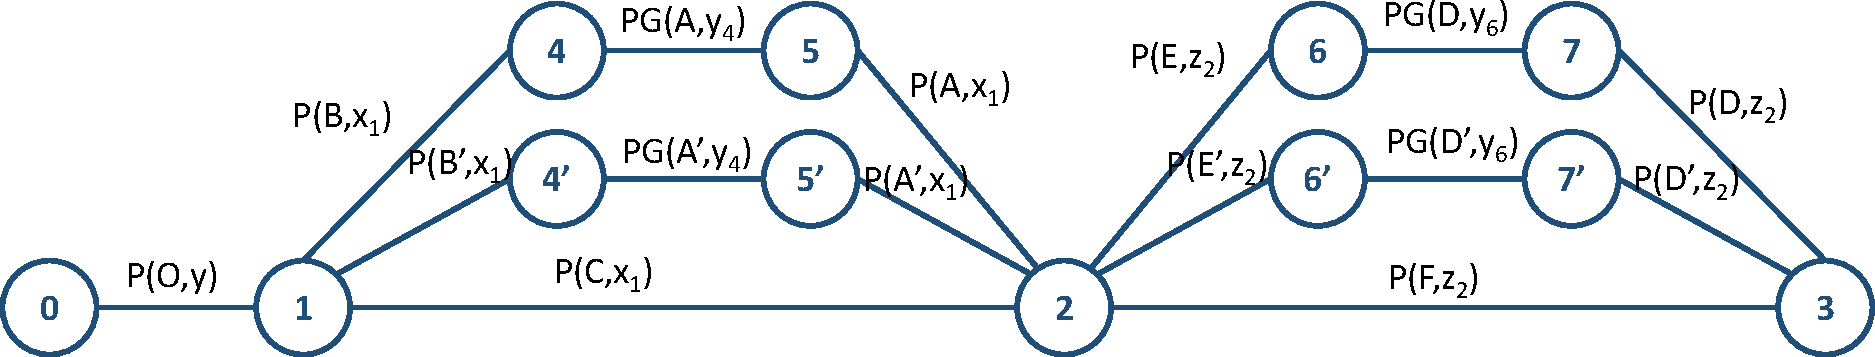
\includegraphics[width=0.9\linewidth]{img/graphe_liaisons}
\end{center}

\paragraph{Question 2:} Calcul d'hyperstatisme:
\begin{itemize}
 \item $12$ pièces dont le bâti,
 \item $11*5+4*4=71$ inconnues de liaison,
 \item le système possède \textbf{trois} mobilité.
\end{itemize}

h=Ns-rs=71-(6*11-3)=71-63=8

~\

\textbf{Le degré d'hyperstatisme du système est 8}.

\paragraph{Question 3:} ~\ \\

\begin{minipage}{0.7\linewidth}
L'architecture du système montre une répétition de la structure des pièces $\left\{1,4,4',5,5',2\right\}$, l'étude de cette partie suffira à conclure pour le reste du mécanisme.
\end{minipage}\hfill
\begin{minipage}{0.25\linewidth}
\begin{center}
 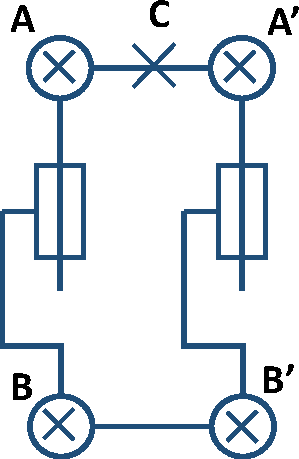
\includegraphics[width=0.6\linewidth]{img/schema_cinematique}
\end{center}
\end{minipage}\hfill

~\

\textbf{Analyse cinématique}

$\left\{V_{2/1}\right\}=\left\{\begin{array}{c c} \omega_{21} & 0 \\ 0 & 0 \\ 0 & 0
\end{array}\right\}_{(C,R_1)}$,
$\left\{V_{4/1}\right\}=\left\{\begin{array}{c c} \omega_{41} & 0 \\ 0 & 0 \\ 0 & 0
\end{array}\right\}_{(B,R_1)}$,
$\left\{V_{4'/1}\right\}=\left\{\begin{array}{c c} \omega_{4'1} & 0 \\ 0 & 0 \\ 0 & 0
\end{array}\right\}_{(B',R_1)}$\\
$\left\{V_{5/4}\right\}=\left\{\begin{array}{c c} 0 & 0 \\ \omega_{54} & V_{54} \\ 0 & 0
\end{array}\right\}_{(A,R_4)}$,
$\left\{V_{5'/4'}\right\}=\left\{\begin{array}{c c} 0 & 0 \\ \omega_{5'4'} & V_{5'4'} \\ 0 & 0\end{array}\right\}_{(A',R_{4'})}$,
$\left\{V_{2/5}\right\}=\left\{\begin{array}{c c} \omega_{25} & 0 \\ 0 & 0 \\ 0 & 0
\end{array}\right\}_{(A,R_1)}$\\
$\left\{V_{2/5'}\right\}=\left\{\begin{array}{c c} \omega_{25'} & 0 \\ 0 & 0 \\ 0 & 0\end{array}\right\}_{(A',R_1)}$.

~\

Tout ramener en C:\\
$\overrightarrow{CB}=\overrightarrow{CO}+\overrightarrow{OB}=-h.\overrightarrow{y_1}+e.\overrightarrow{z_1}$\\
$\overrightarrow{CB'}=\overrightarrow{CO}+\overrightarrow{OB'}=-h.\overrightarrow{y_1}-e.\overrightarrow{z_1}$\\
$\overrightarrow{CA}=e.\overrightarrow{z_2}=e.(-sin\theta_2.\overrightarrow{y_1}+cos\theta_2.\overrightarrow{z_1})$\\
$\overrightarrow{CA'}=-e.\overrightarrow{z_2}=-e.(-sin\theta_2.\overrightarrow{y_1}+cos\theta_2.\overrightarrow{z_1})$

$\left\{V_{2/1}\right\}=\left\{\begin{array}{c c} \omega_{21} & 0 \\ 0 & 0 \\ 0 & 0
\end{array}\right\}_{C,R_1}$,
$\left\{V_{4/1}\right\}=\left\{\begin{array}{c c} \omega_{41} & 0 \\ 0 & e.\omega_{41} \\ 0 & h.\omega_{41} 
\end{array}\right\}_{C,R_1}$\\
$\left\{V_{4'/1}\right\}=\left\{\begin{array}{c c} \omega_{4'1} & 0 \\ 0 & -e.\omega_{4'1} \\ 0 & h.\omega_{4'1} 
\end{array}\right\}_{C,R_1}$,

$\left\{V_{5/4}\right\}=\left\{\begin{array}{c c} 0 & -e.cos(\theta_2-\theta_4).\omega_{54} \\ cos\theta_4.\omega_{54} & cos\theta_4.V_{54} \\ sin\theta_4.\omega_{54} & sin\theta_4.V_{54} \end{array}\right\}_{(C,R_1)}$,
$\left\{V_{5'/4'}\right\}=\left\{\begin{array}{c c} 0 & e.cos(\theta_2-\theta'_4).\omega_{5'4'} \\ cos\theta'_4.\omega_{5'4'} & cos\theta'_4.V_{5'4'} \\ sin\theta'_4.\omega_{5'4'} & sin\theta'_4.V_{5'4'} \end{array}\right\}_{(C,R_1)}$,
$\left\{V_{2/5}\right\}=\left\{\begin{array}{c c} \omega_{25} & 0 \\ 0 & e.cos\theta_2.\omega_{25} \\ 0 & e.sin\theta_2.\omega_{25}\end{array}\right\}_{(C,R_1)}$,
$\left\{V_{2/5'}\right\}=\left\{\begin{array}{c c} \omega_{25'} & 0 \\ 0 & -e.cos\theta_2.\omega_{25'} \\ 0 & -e.sin\theta_2.\omega_{25'}\end{array}\right\}_{(C,R_1)}$.

$\left\{\begin{array}{l} \omega_{21}=\omega_{25}+\omega_{41}=\omega_{25'}+\omega_{4'1} \\
0=cos\theta_4.\omega_{54}=cos\theta'_4.\omega_{5'4'} \\ 0=sin\theta_4.\omega_{54}=sin\theta'_4.\omega_{5'4'} \\ 0=-e.cos(\theta_2-\theta_4).\omega_{54}=-e.cos(\theta_2-\theta'_4).\omega_{5'4'} \\ 0=e.cos\theta_2.\omega_{25}+cos\theta_4.V_{54}+e.\omega_{41}=-e.cos\theta_2.\omega_{25'}+cos\theta'_4.V_{5'4'}-e.\omega_{4'1} \\ 0=e.sin\theta_2.\omega_{25}+sin\theta_4.V_{54}+h.\omega_{41}=-e.sin\theta_2.\omega_{25'}+sin\theta'_4.V_{5'4'}+h.\omega_{4'1}
\end{array}\right.$

~\

Analyse des équations:
\begin{itemize}
 \item à la ligne 2, ont sait que $\omega_{54}=0$ et $\omega_{5'4'}=0$,
 \item ces informations apparaissent aux lignes 3 et 4,
 \item \textbf{4} degrés d'hyperstatisme dans les deux cycles, soit un total de \textbf{8}.
\end{itemize}

\end{document}
